\section{Návrh a výroba desky plošných spojů}
\subsection{Návrh DPS}
Pro návrh DPS byl využit svobodný software KiCAD. Součástky a jejich propojení
jsou importovány ze schématu, jejich rozmístění na DPS a propojení cestami ale
musí provést člověk.

Před generováním návrhu plošného spoje je vhodné ověřit správnost schématu
nástrojem ERC (Electrical Rules Checker).

\begin{figure}[htbp]
    \centering
    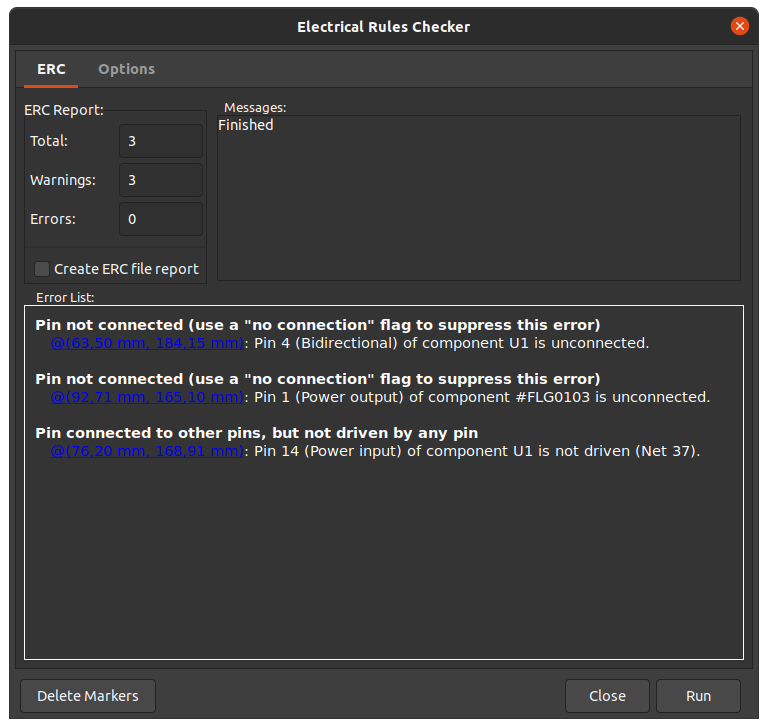
\includegraphics[width=0.70\textwidth]{KICAD-ERC}
    \caption{Výsledek kontroly ERC s několika detekovanými chybami}
    \label{fig:kicad ERC}
\end{figure}

\begin{figure}[htbp]
    \centering
    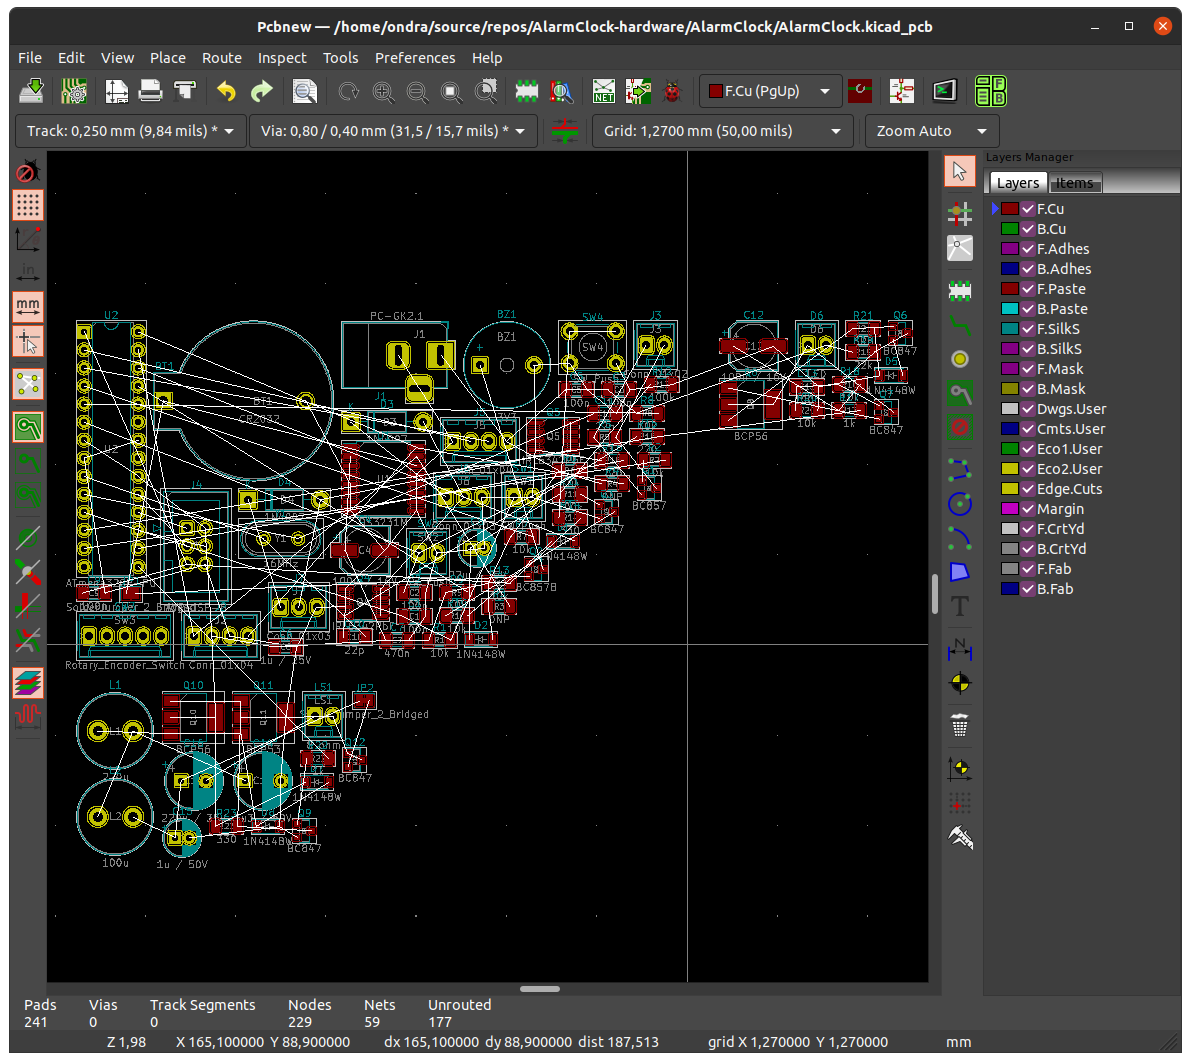
\includegraphics[width=0.80\textwidth]{KICAD-po-importu}
    \caption{%
        Nástroj pro návrh DPS \shellcmd{pcbnew} po importu součástek ze
        schématu
    }
    \label{fig:kicad po importu}
\end{figure}

Nástroj pro kontrolu správnosti návrhu plošného spoje se nazývá DRC. Ten
kontroluje, zda-li je možné DPS vyrobit procesem s definovanými vlastnostmi
(minimální šířka cesty, minimální izolační mezera, ...). Pro proces frézování
je vhodné používat poměrně široké cesty~-- \SI{1}{\milli\meter} pro většinu
spojů, \SI{0,8}{\milli\meter} pro cesty propojující SMD integrované obvody.

DPS byla navržena tak, aby ji bylo možné vyrobit s mědí z jedné strany či
oboustranně. Na jednostranném plošném spoji jsou cesty na horní měděné vrstvě
nahrazeny drátovými propojkami.

Úplné schéma zapojení a návrh DPS jsou otištěny v příloze~\ref{app:PCB}.


\subsection{Výroba DPS}
Pro výrobu prototypů desek plošných spojů lze využít metodu vytváření
izolačních mezer v měděné vrstvičce pomocí CNC frézy. Jde o poměrně rychlou
metodu s minimem manuální práce. Stroj navíc provádí i navrtání děr, jejichž
počet i na poměrně jednoduchých DPS využívajících v maximální možné míře
součástek pro povrchovou montáž dosahuje několika stovek. Celý proces se obejde
bez nutnosti pracovat s korozivními chemikáliemi. Frézování oboustranných DPS
je možné, v takovém případě se ale zvyšuje náročnost postupu. Je totiž nutné
zachovat pozici referenčního bodu při otáčení desky.

\subsubsection{CNC fréza}
Levným CNC strojem splňujícím požadavky na přesnost, rozměry pracovního
prostoru a podporované funkce vhodným pro amatérské účely je stavebnice
prodávaná prodejci na platformě Aliexpress pod označením CNC~1610. Je tvořena
konstrukcí z hliníkových profilů a několika 3D tištěných částí. Po sestavení
získává uživatel stroj s pracovním prostorem \SI{160 x 100 x 40}{\milli\meter}
řízený svobodným firmware Grbl\footnote{\url{https://github.com/gnea/grbl}}.

\begin{figure}[htbp]
    \centering
    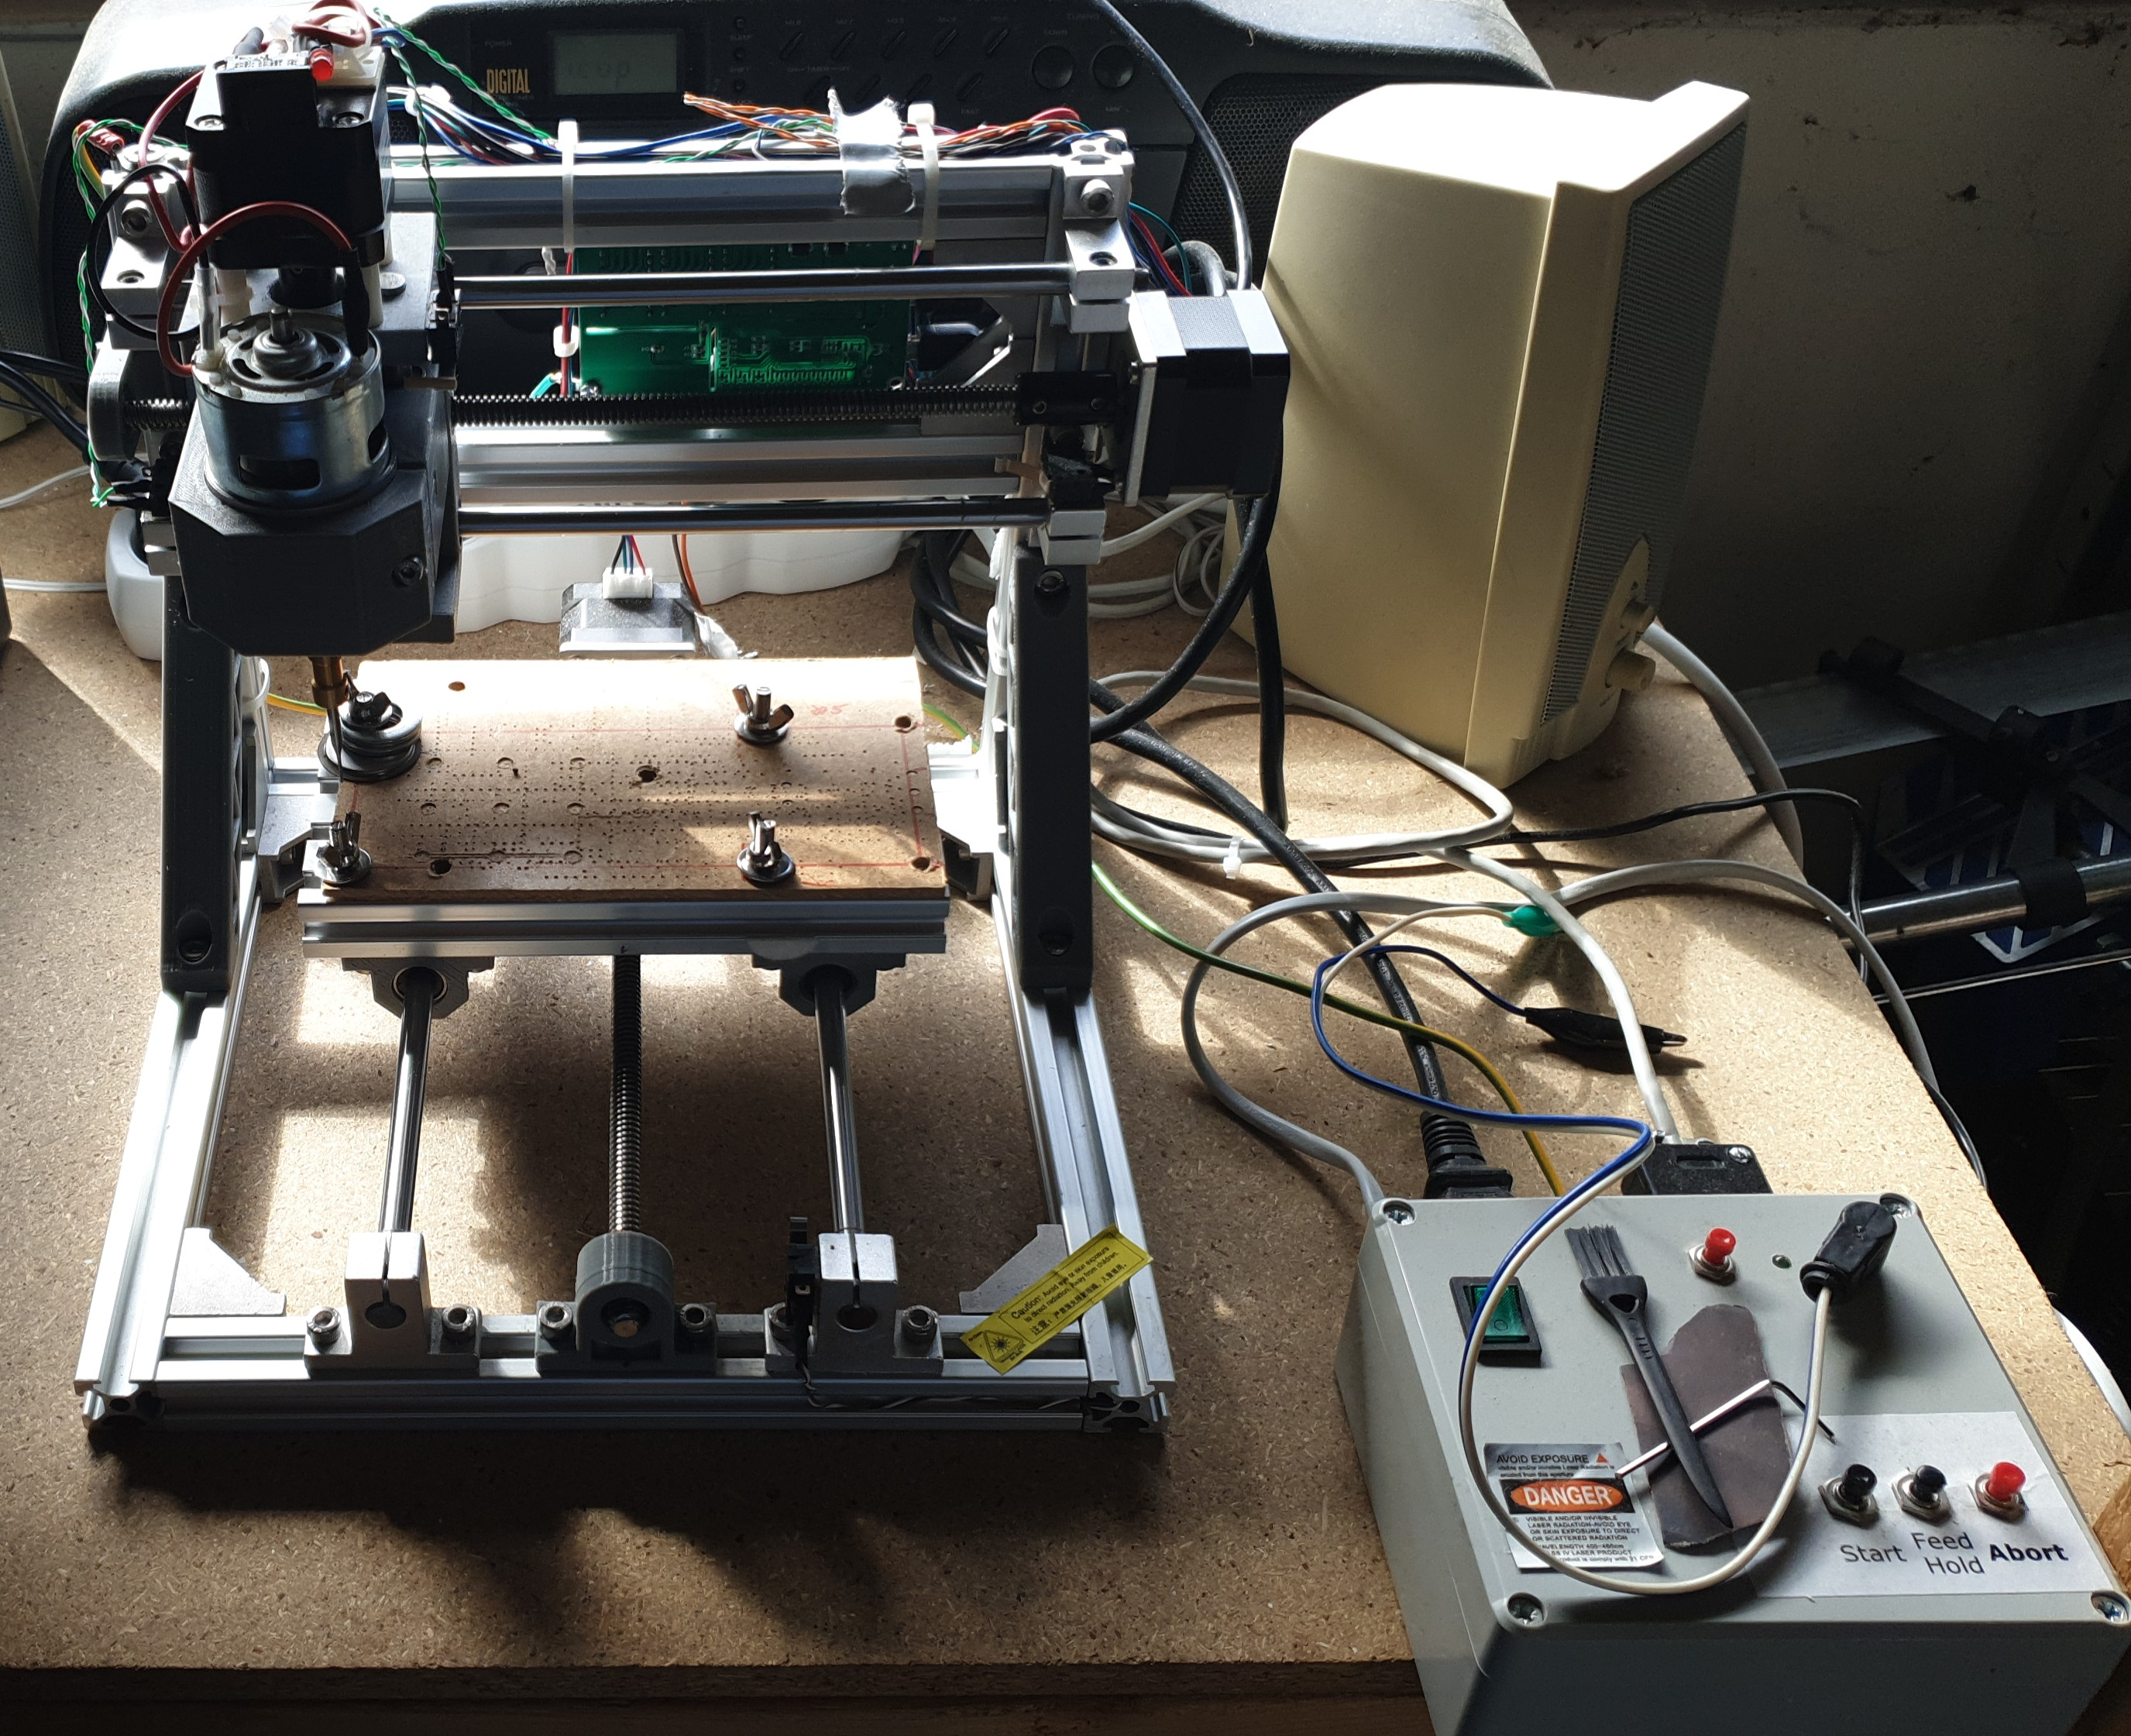
\includegraphics[width=1.0\textwidth]{CNC-freza}
    \caption{CNC fréza CNC~1610 s drobnými úpravami}
    \label{fig:CNC freza}
\end{figure}


\paragraph{Modifikace}
Po zakoupení stroje byly provedeny některé modifikace, které nadále
zjednodušují proces výroby DPS. Jednou z nich je přidání koncových spínačů.
Jejich funkce je dvojí. Zvyšují bezpečnost, protože zabraňují nárazu
pohyblivých částí stroje do jeho rámu (v případě využití
\foreignlanguage{english}{homing cycle} dokonce nemusí nutně dojít ani
k sepnutí tohoto spínače, pohyb mimo pracovní prostor je detekován výpočetně).
Umožňují také provést po spuštění stroje kalibraci
(\foreignlanguage{english}{homing cycle}), po které odpovídají souřadnice
stroje (v Grbl zvané \foreignlanguage{english}{machine coordinates})
konkrétním bodům v jeho pracovním prostoru. Díky tomu je možné beze ztráty
přesnosti obnovit práci například po výpadku napájení.

Druhá modifikace je pro výrobu DPS ještě důležitější. Jde o přidání kabelů
s krokosvorkami na vstup pro sondu (\foreignlanguage{english}{probe}). Jedna ze
svorek je spojena s měděnou vrstvou obráběné DPS, druhá je připojena na
frézovací nástroj upnutý v zastaveném vřetenu. Stroj díku tomu může přesně
změřit výšku desky v různých bodech a kompenzovat tak její průhyby. Vlastní
frézování je totiž velmi mělké, méně než \SI{200}{\micro\meter}.

\begin{figure}[htbp]
    \centering
    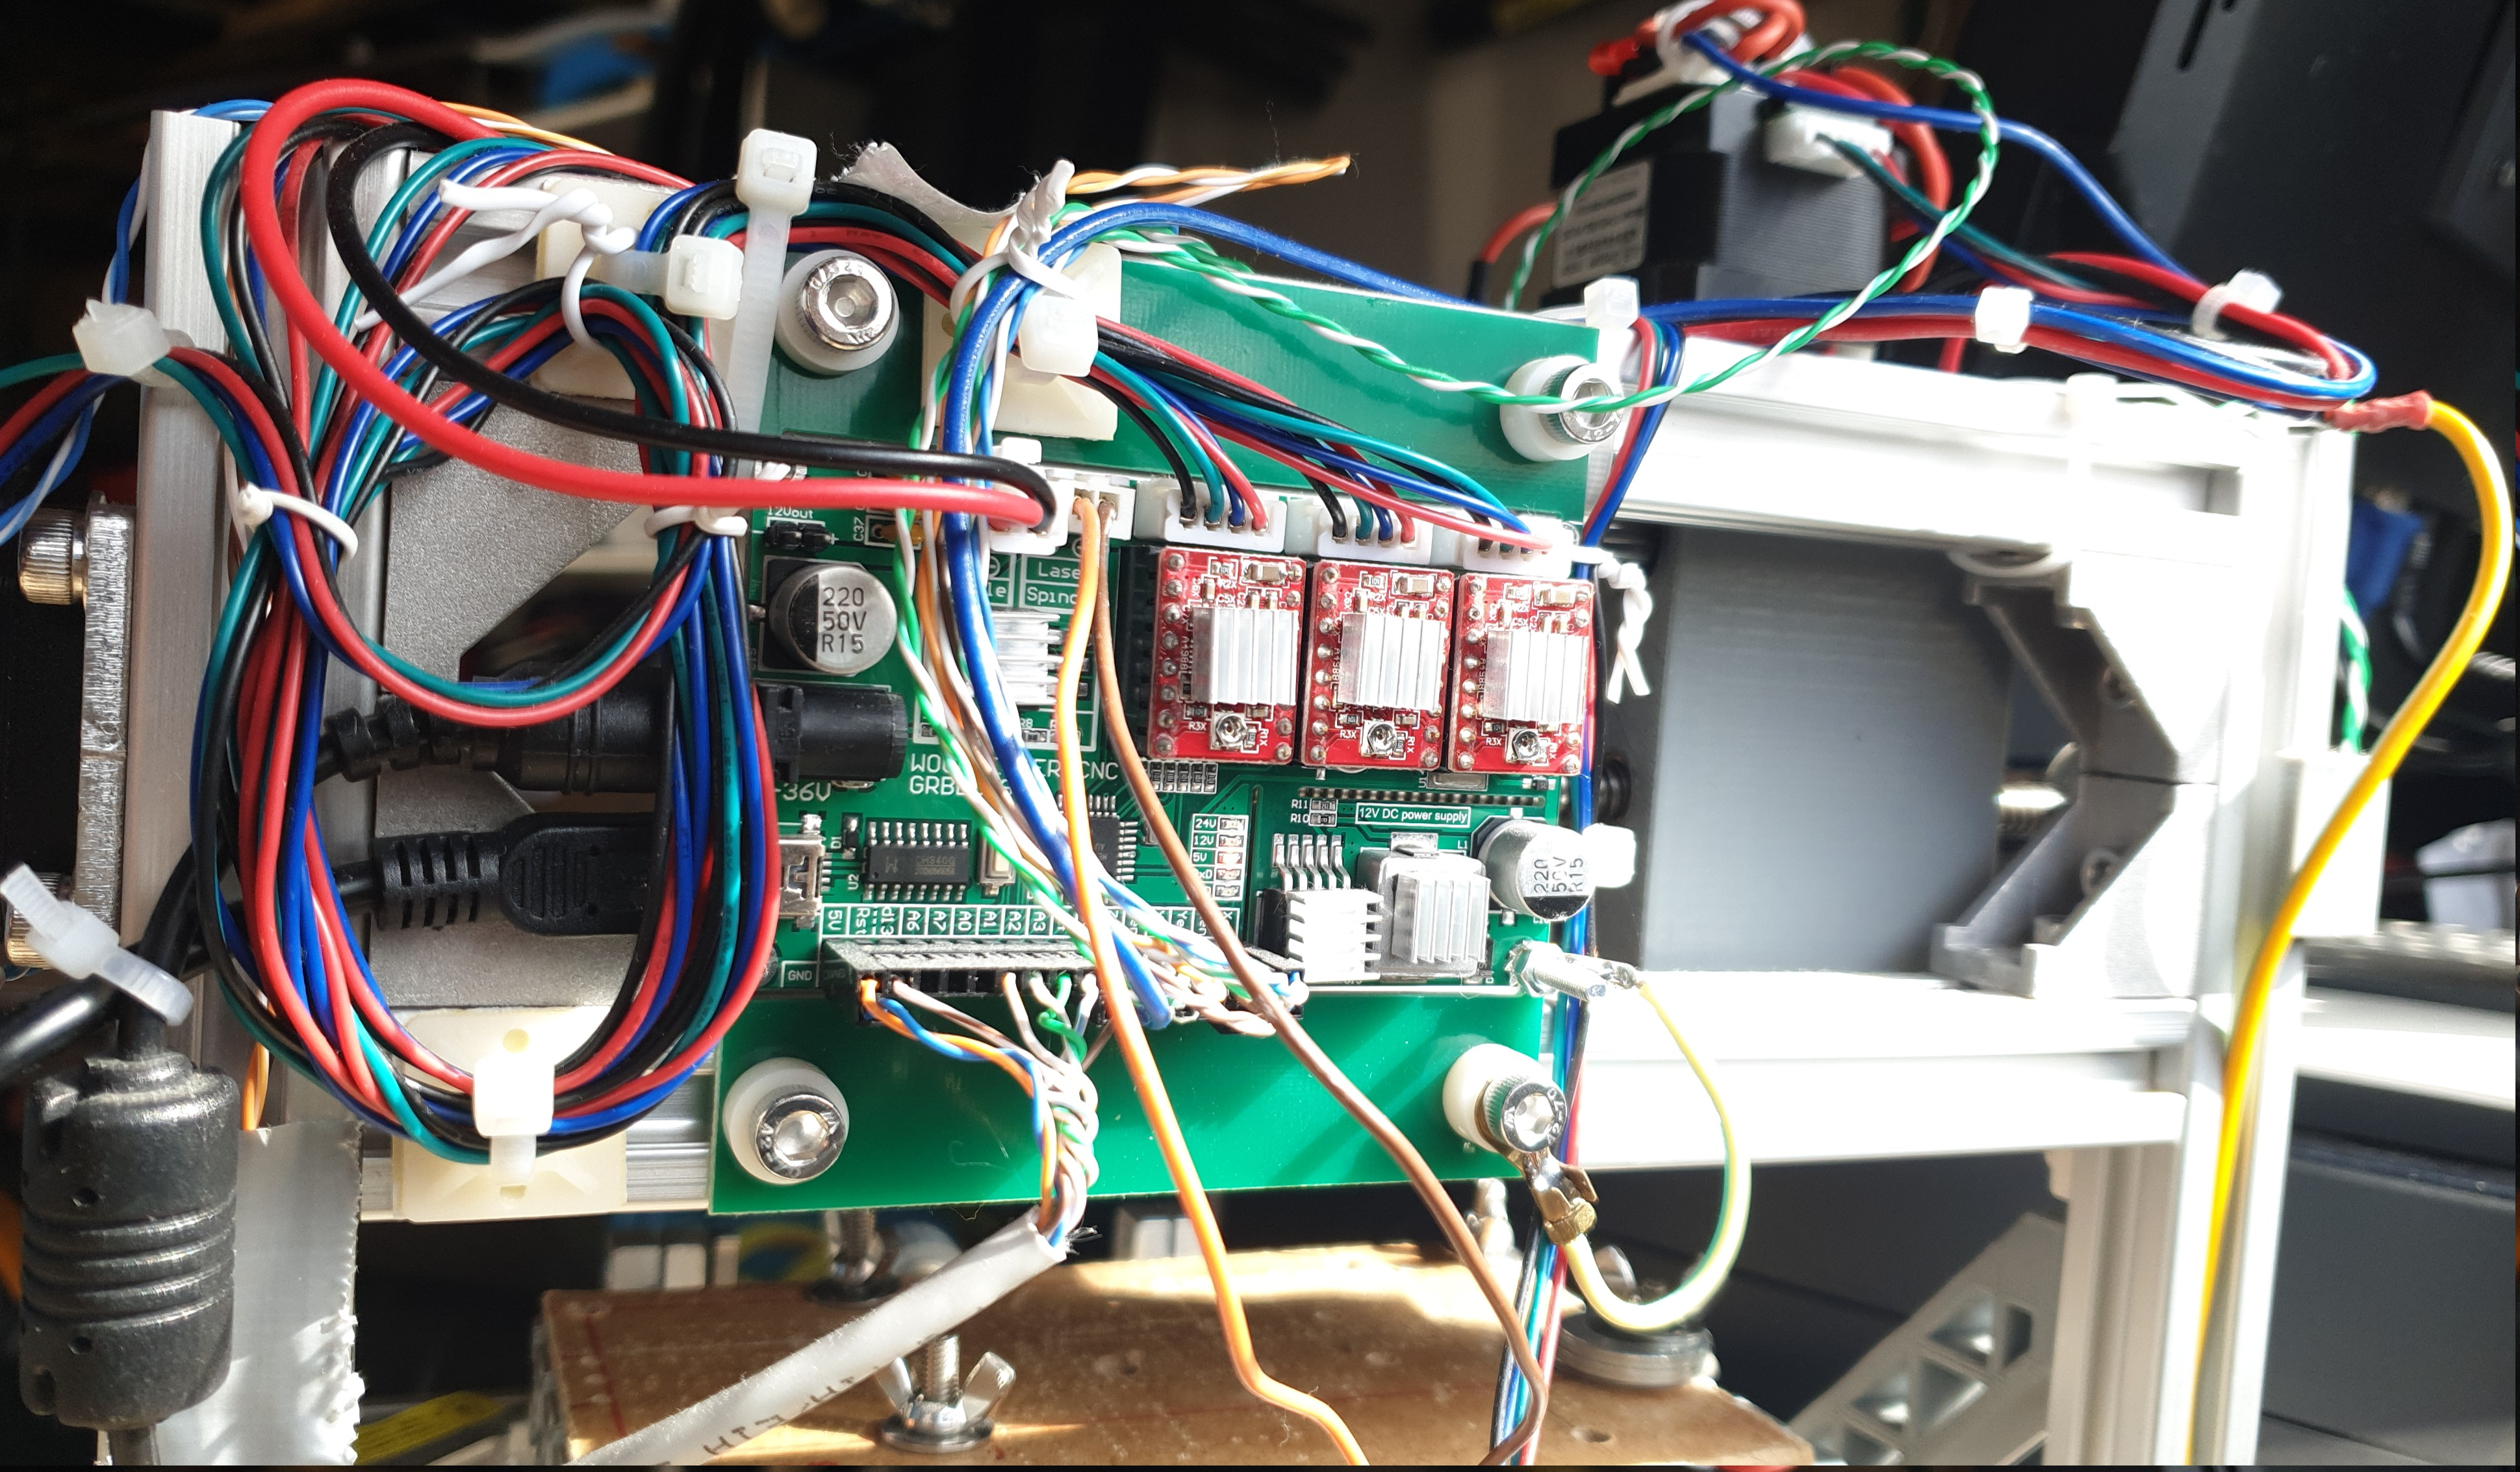
\includegraphics[width=1.0\textwidth]{CNC-rizeni}
    \caption{%
        Řídicí elektronika CNC frézy s připojenými koncovými spínači a~sondou
    }
    \label{fig:CNC rizeni}
\end{figure}

Po provedení modifikací je nutné správně změnit nastavení Grbl, zejména
\verb|$5|, \verb|$6|, \verb|$20|, \verb|$21| a \verb|$22| až \verb|$27|.
Je také nutné správně nastavit rozměry pracovního prostoru (\verb|$130| až
\verb|$132|), protože výrobce toto nastavení ignoruje a ponechává jej na
výchozí hodnotě. Úplná konfigurace Grbl včetně vysvětlení jednotlivých
nastavení je otištěna v příloze~\vref{app:grbl config}.

Aby bylo možné využívat novější verzi řídicího software (spouštěného na
počítači), je nutné aktualizovat firmware stroje z verze Grbl~0.9j na
Grbl~1.1h. Aktualizace se provádí dle instrukcí na domovské stránce projektu
Grbl pomocí Arduino IDE. Přečtením obsahu paměti FLASH s původním firmware bylo
zjištěno, že použitý bootloader odpovídá desce \uv{Arduino nano (old
bootloader)}. Před aktualizací je vhodné vytvořit zálohu původního obsahu
paměti. To lze na počítači s operačním systémem GNU/Linux s nainstalovaným
Arduino IDE provést následujícím příkazem:
\begin{lstlisting}[style=terminal]
$ $HOME/.arduino15/packages/arduino/tools/avrdude/6.3.0-arduino17/bin/avrdude \
    -C$HOME/.arduino15/packages/arduino/tools/avrdude/6.3.0-arduino17/etc/avrdude.conf \
    -v -patmega328p -carduino -P/dev/ttyUSB0 -b5 7600 -D \
    -Uflash:r:$HOME/Desktop/CNC/GRBL-old-read.bin:r
\end{lstlisting}
Dále je nutné zazálohovat nastavení Grbl, která jsou uložená v paměti EEPROM.
To se provádí připojením terminálu na sériový port stroje a spuštěním příkazu
\verb|$$|.
Po aktualizaci firmware je potřeba nová nastavení stroje porovnat s touto
zálohou a příslušně je upravit.

\paragraph{Nástroje}
Pro frézování obrazce DPS jsou vhodné nástroje ve tvaru V. Průměr nástroje
v místě upnutí je \SI{3,175}{\milli\meter}, to je standardní rozměr používaný
na malých CNC frézách. Nástroj se poté zužuje s úhlem
\SI{15}{\degree} až k velmi tenkému hrotu.

Pro vrtání děr využíváme tvrzené vrtáky o průměru \SI{0,8}{\milli\meter}
a \SI{1}{\milli\meter}. Tyto dva rozměry postačí pro naprostou většinu běžných
DPS. Montážní díry o průměru \SI{3,2}{\milli\meter} se tímto vrtákem předvrtají
a na požadovaný průměr je zvětšíme stojanovou vrtačkou. Drážky pro vývody
napájecího konektoru lze vyfrézovat frézou \uv{corn bit} o průměru
\SI{1}{\milli\meter}. Stejným nástrojem je provedeno i oddělení hotové DPS od
zbytku materiálu.

\begin{figure}[htbp]
    \centering
    \subcaptionbox{%
        V-bit a fréza \SI{1}{\milli\meter}
    }[0.3\textwidth]{%
        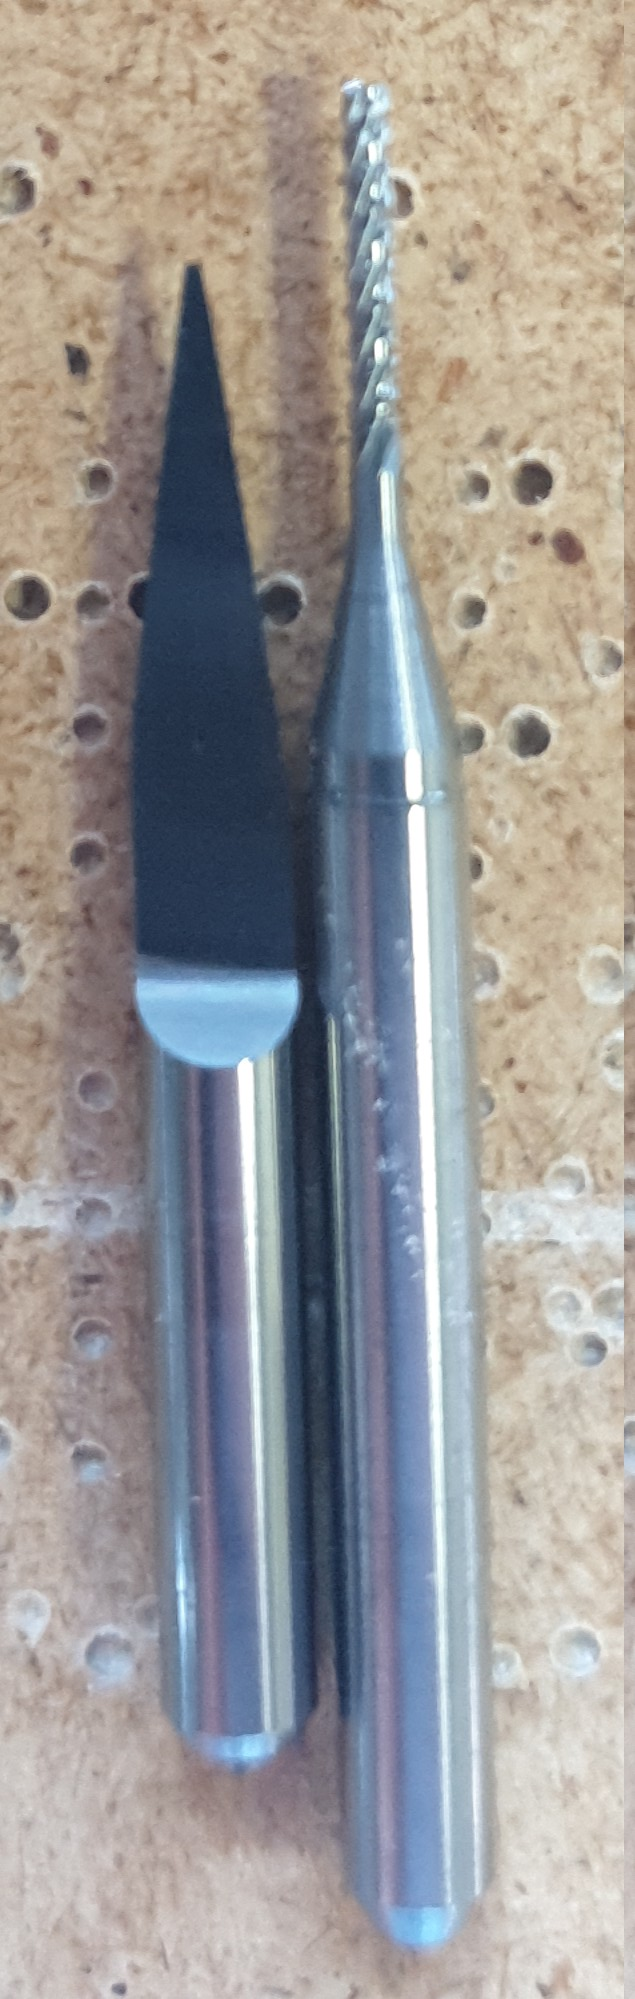
\includegraphics[height=50mm]{CNC-nastroj-V-freza}
    }
    \subcaptionbox{%
        Vrták \SI{0,8}{\milli\meter}
    }[0.3\textwidth]{%
        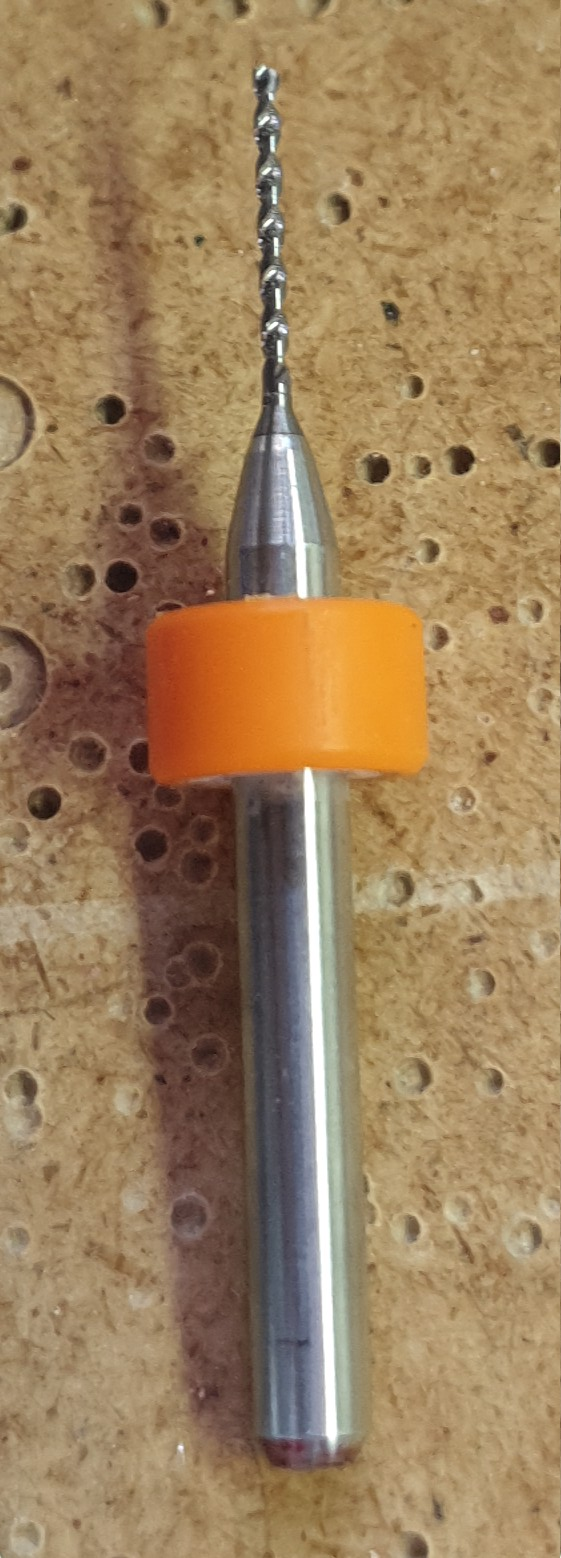
\includegraphics[height=50mm]{CNC-nastroj-08}
    }
    \subcaptionbox{%
        Vrták \SI{1,0}{\milli\meter}
    }[0.3\textwidth]{%
        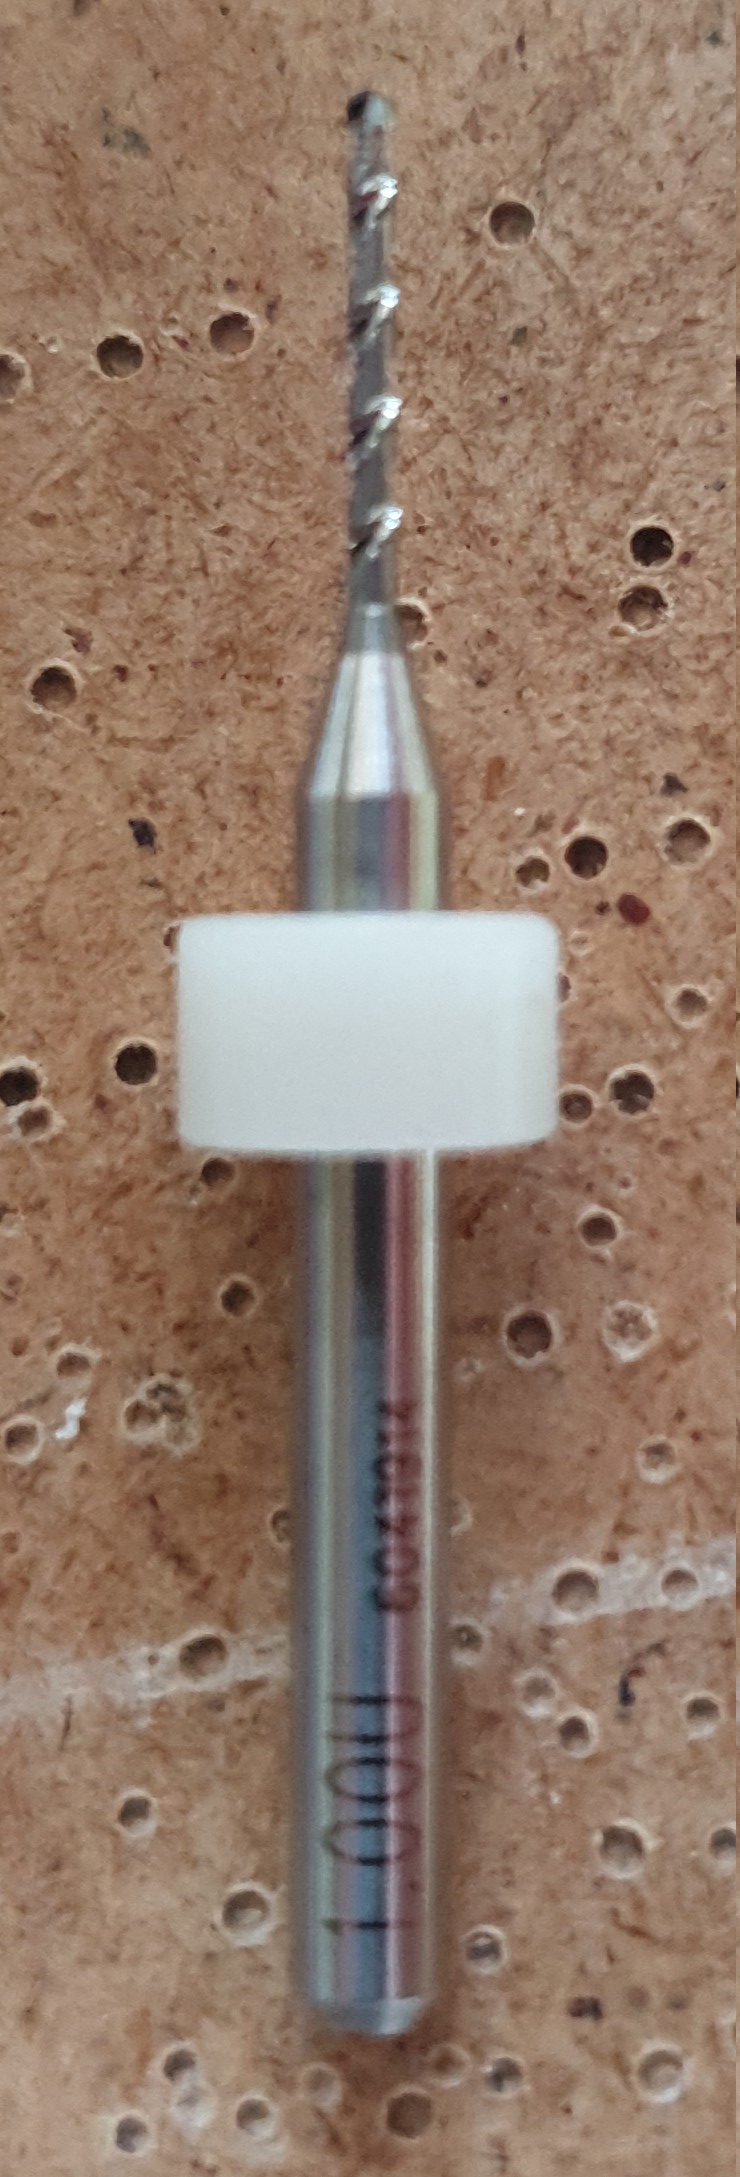
\includegraphics[height=50mm]{CNC-nastroj-10}
    }
    \caption{Nástroje používané při frézování DPS}
    \label{fig:CNC nastroje}
\end{figure}

\begin{figure}[htbp]
    \centering
    \includegraphics[width=0.65\textwidth]{CNC-drazky-nastroj}
    \hfill
    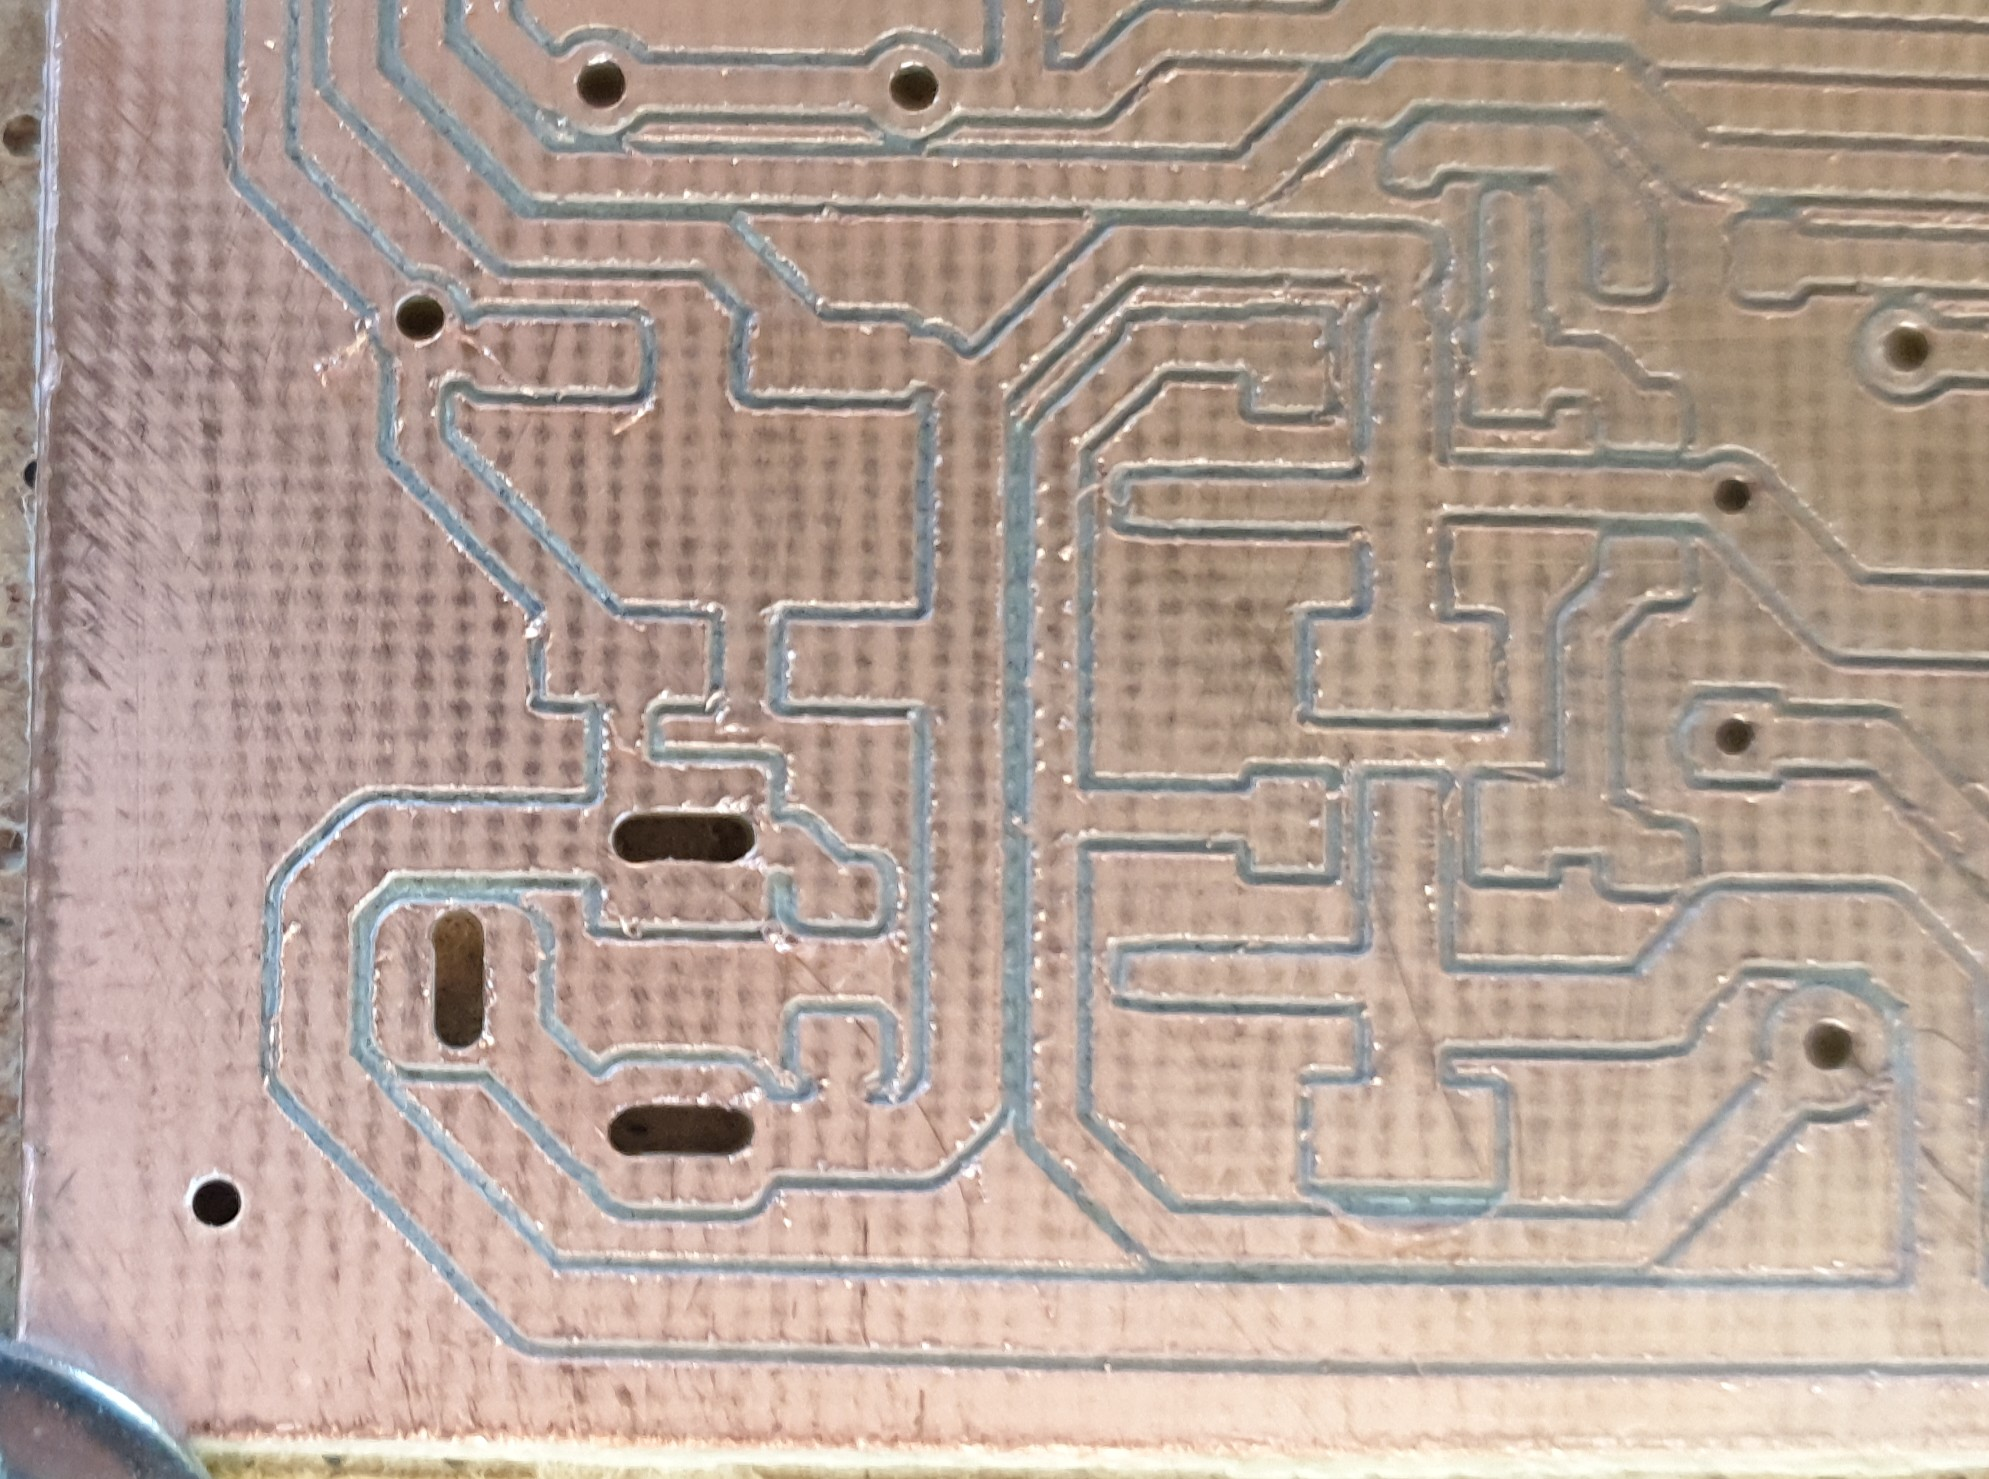
\includegraphics[width=0.25\textwidth]{CNC-drazky}
    \caption{Frézování drážek pro vývody napájecího konektoru}
    \label{fig:CNC drazky}
\end{figure}

\begin{figure}[htbp]
    \centering
    \includegraphics[width=0.80\textwidth]{CNC-outline}
    \caption{Frézování okraje DPS}
    \label{fig:CNC outline}
\end{figure}


\paragraph{Řídicí software}
Řízení vlastního stroje (krokových motorů a vřetena) je řešeno mikrokontrolérem
na jeho desce s řídicí elektronikou. Jeho firmware Grbl implementuje jazyk
G-kód, příkazy jsou přijímány na sériovém portu. Tyto příkazy by bylo možné
zasílat z běžného terminálu, pro zvýšení pohodlí při obsluze stroje je ale
vhodné využít specializovaný software. Jedním z takových programů je
Candle\footnote{\url{https://github.com/Denvi/Candle}}. Jde o svobodný software
distribuovaný pod licencí GNU GPL v3.0. Kromě GNU/Linux je podporován
i operační systém Microsoft Windows. Uživatelské rozhraní tohoto programu (viz
obrázek~\vref{fig:CNC Candle} velmi dobře funguje s dotykovým monitorem.
Jednoduché operace je možné provádět přímo dedikovanými tlačítky či klávesovými
zkratkami, složitější příkazy je možné vypisovat přímo do okna \uv{Console}.

% Stabilní verze z větve \gitbranch{master} je již poměrně stará, proto je
% využívána vývojová verze z větve \gitbranch{Experimental}.
% https://github.com/Denvi/Candle/issues/488#issuecomment-858985048

\begin{figure}[htbp]
    \centering
    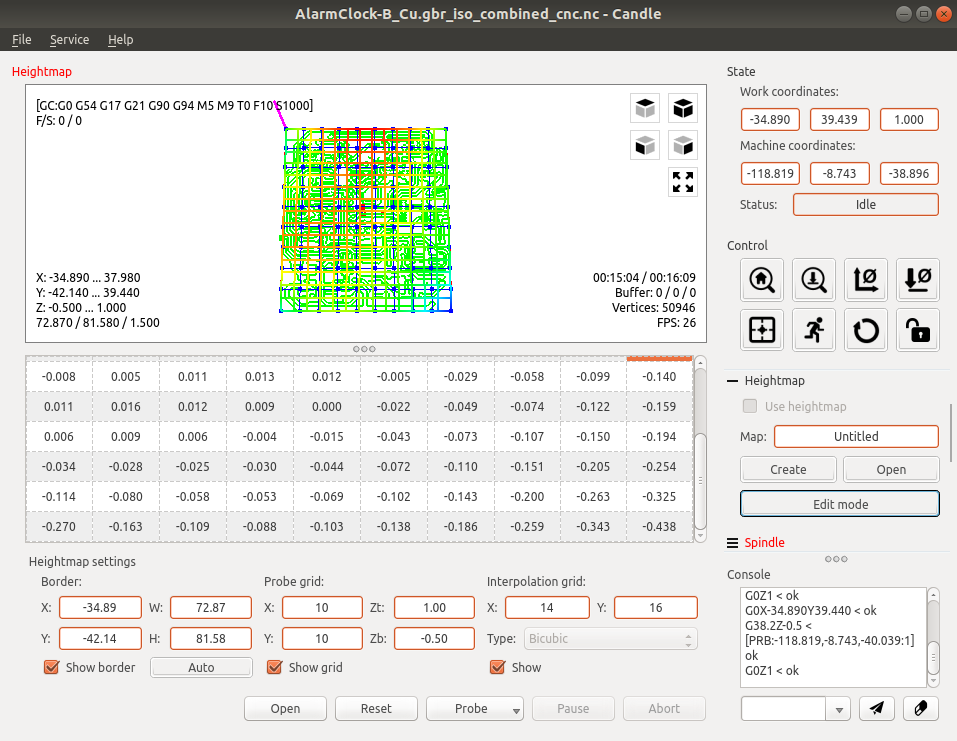
\includegraphics[width=\textwidth]{Candle-UI}
    \caption{Uživatelské rozhraní programu Candle}
    \label{fig:CNC Candle}
\end{figure}


\subsubsection{Generování G-kódu}
G-kód lze psát ručně pomocí běžného textového editoru. Mnohdy je to dokonce
nejrychlejší metoda. Jednoduché operace, jako například vyříznutí hotové DPS
z větší cuprextitové destičky, obvykle sestávají z méně než 15 příkazů
a operátor se základní znalostí G-kódu je zvládne vytvořit velmi rychle.
Složitější operace, jako například frézování vlastního obrazce DPS, ale
vyžadují desítky tisíc příkazů a jejich ruční tvorba by byla prakticky nemožná.
Existuje ale svobodný software FlatCAM\footnote{\url{http://flatcam.org/}},
který slouží k automatickému generování G-kódu z podkladů ve formátu Gerber.
Úplný popis postupu práce s tímto software by byl nad rámec této práce, soubor
FlatCAM projektu je ale součástí elektronické přílohy (viz
příloha~\vref{app:dirtree}).

\begin{figure}[htbp]
    \centering
    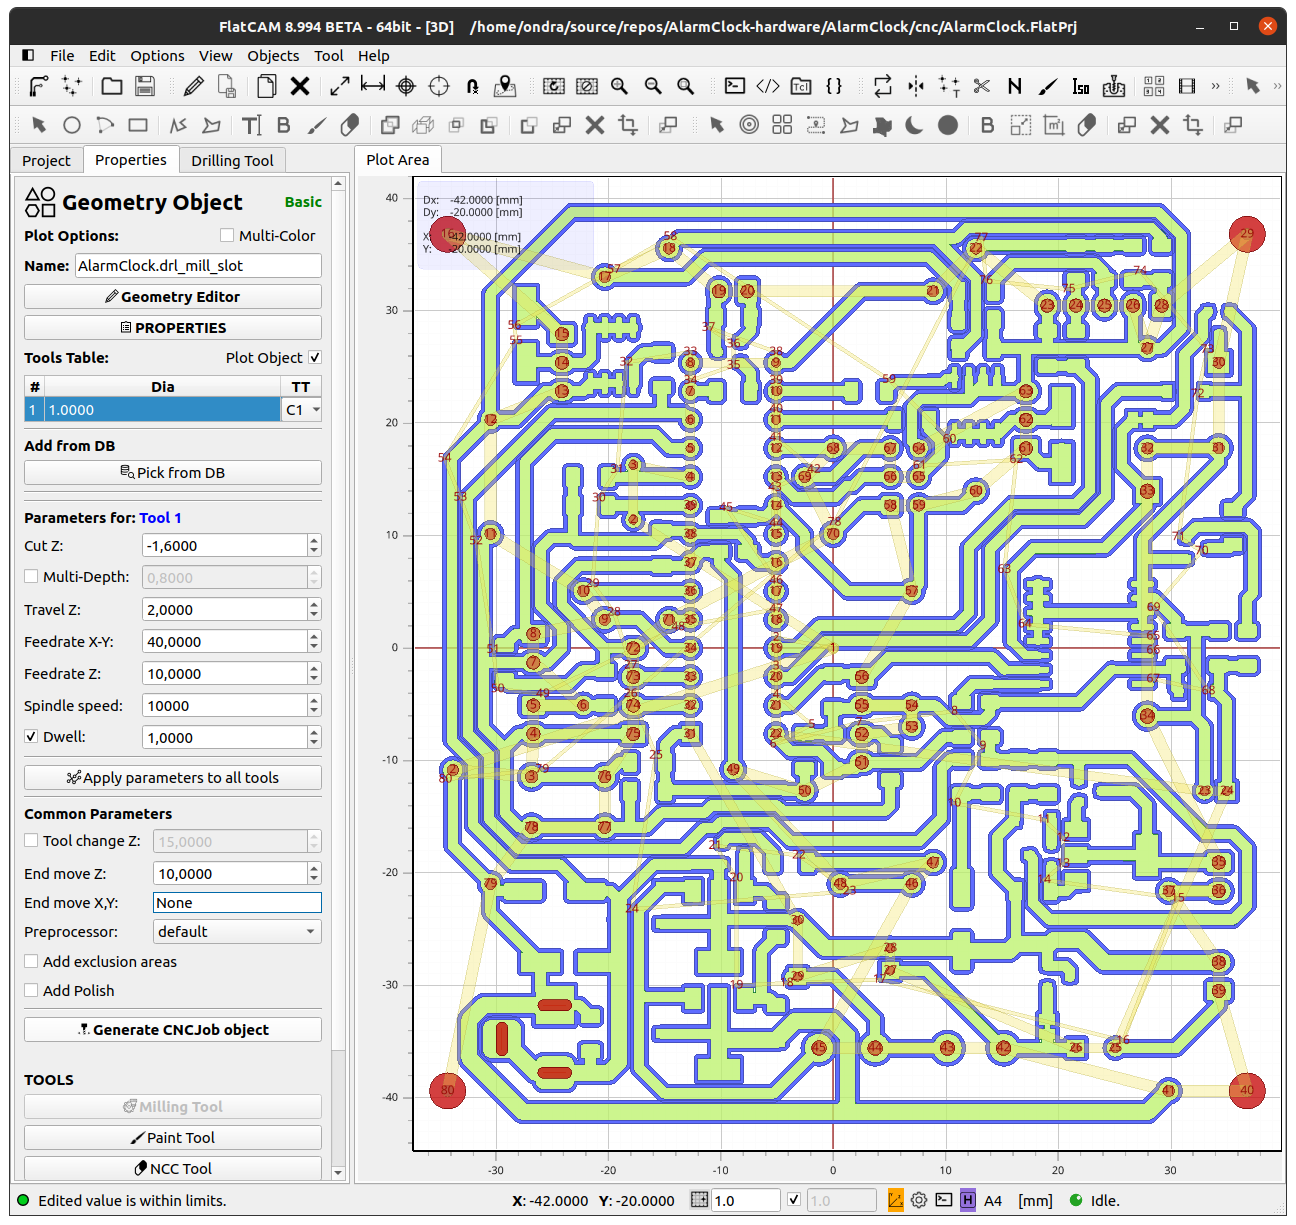
\includegraphics[width=\textwidth]{FlatCAM-GUI}
    \caption{Uživatelské rozhraní software FlatCAM}
    \label{fig:CNC FlatCAM}
\end{figure}


\subsection{Osazování DPS}
Pro osazování součástek pro povrchovou montáž na DPS vyrobenou procesem
frézování nelze využít pájení horkým vzduchem po aplikaci pájecí pasty, protože
by pravděpodobně došlo k nechtěnému připájení součástek k neodfrézované ploše
mědi. Všechny součástky jsou proto pájeny ručně.

\begin{figure}[htb]
    \centering
    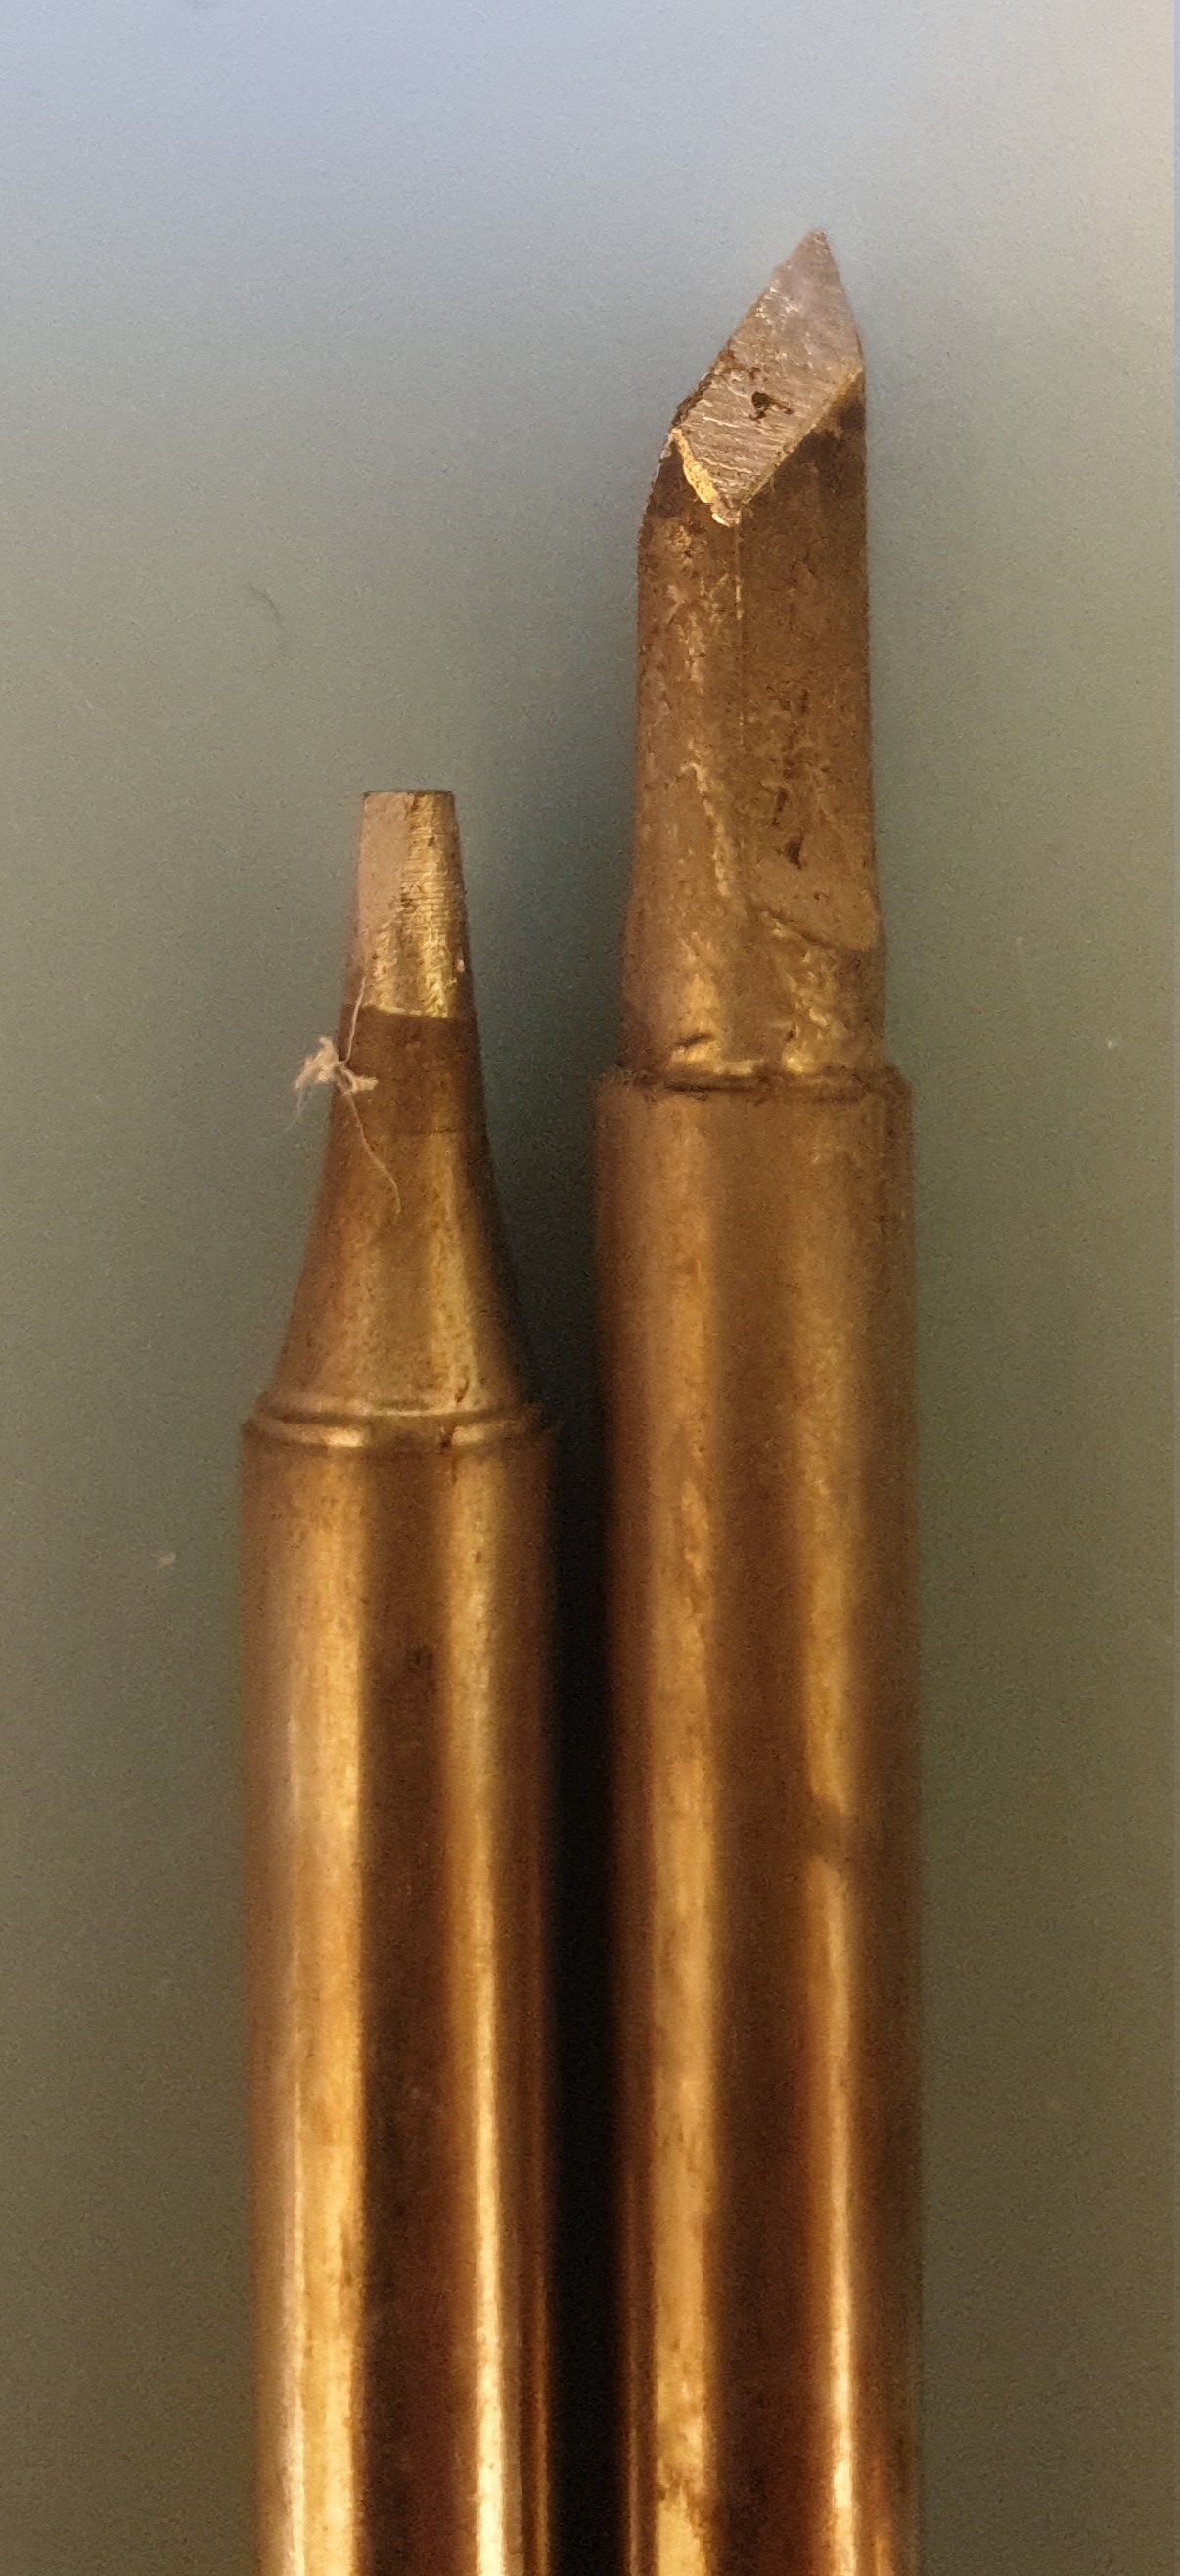
\includegraphics[width=0.45\textwidth,height=60mm,keepaspectratio]{T12-hroty-detail}
    \\
    {\footnotesize Nalevo T12-D16 používaný pro pájení SMD součástek;
    napravo T12-K používaný pro pájení THT součástek.}
    \caption{Hroty pro pájecí stanici T12 používané při osazování DPS}
    \label{fig:PCB pajecka hroty}
\end{figure}

Nejprve osazujeme součástky pro povrchovou montáž (SMT) na spodní straně DPS.
Abychom zabránili poškození polovodičových součástek elektrostatickými výboji,
provádíme osazování a pájení na antistatické podložce. Technik pracující na DPS
by měl nosit antistatický náramek. Je také vhodné nejdříve osazovat pasivní
součástky, aby se riziko poškození polovodičových součástek dále zmenšilo.

Součástky pro THT montáž osazujeme od nejnižších po nejvyšší. Na místo
mikrokontroléru (U2) je vhodné připájet patici, do které se integrovaný obvod
vloží. Pokud byl plošný spoj vyroben jako jednostranný, je nutné vyrobit
a připájet několik drátových propojek.

Při osazování je výhodné využít interaktivní osazovací plán, který je generován
pluginem do KiCAD zvaným
\texttt{InteractiveHtmlBom}\footnote{\url{https://github.com/openscopeproject/InteractiveHtmlBom}}.
Pro jeho zobrazení je využit webový prohlížeč, ve kterém se otevře soubor
\repopath{AlarmClock/bom/ibom.html} z repozitáře \gitrepo{AlarmClock-hardware}.

\begin{figure}[htbp]
    \centering
    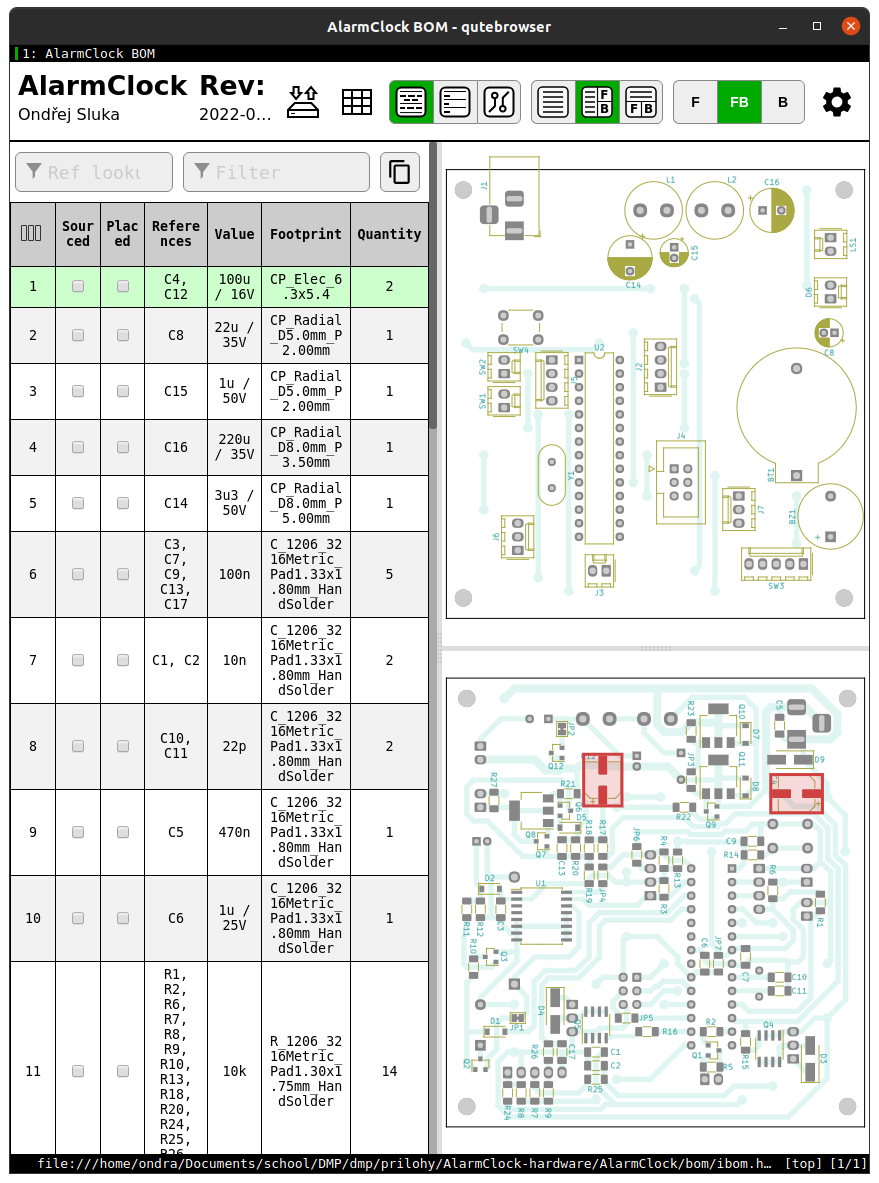
\includegraphics[width=\textwidth]{KICAD-ibom}
    \caption{Interaktivní osazovací plán}
    \label{fig:PCB ibom}
\end{figure}


\subsubsection{Modifikace modulu I/O expandéru}
Pro připojení LCD je využit komerčně dostupný modul s I/O expandérem PCF8574.
Ten je ale nutné před připájením na zadní stranu LCD upravit. Obsahuje totiž
pull-up rezistory na sběrnici \IIC{}, které by po jeho připojení tvořily
paralelní kombinaci s rezistory na hlavní DPS. Modul také obsahuje červenou SMD
LED, která po připojení napájení neustále svítí.

Modifikace spočívá v odpájení 3 SMD rezistorů v pouzdře 0805. Rezistory jsou
umístěny těsně vedle sebe, další blízkou součástkou je právě LED dioda. Tu není
nutné odpájet, protože z obvodu odstraníme její předřadný rezistor R10
(\SI{1}{\kilo\ohm}), ale pokud k jejímu poškození dojde omylem, nezmění se nic
na funkci modulu. Pull-up rezistory R8 a R9 mají hodnotu \SI{4,7}{\kilo\ohm}.
Úpravu lze snadno provést horkovzdušnou stanicí.

\begin{figure}[htbp]
    \centering
    \subcaptionbox{Modul před modifikací}{%
        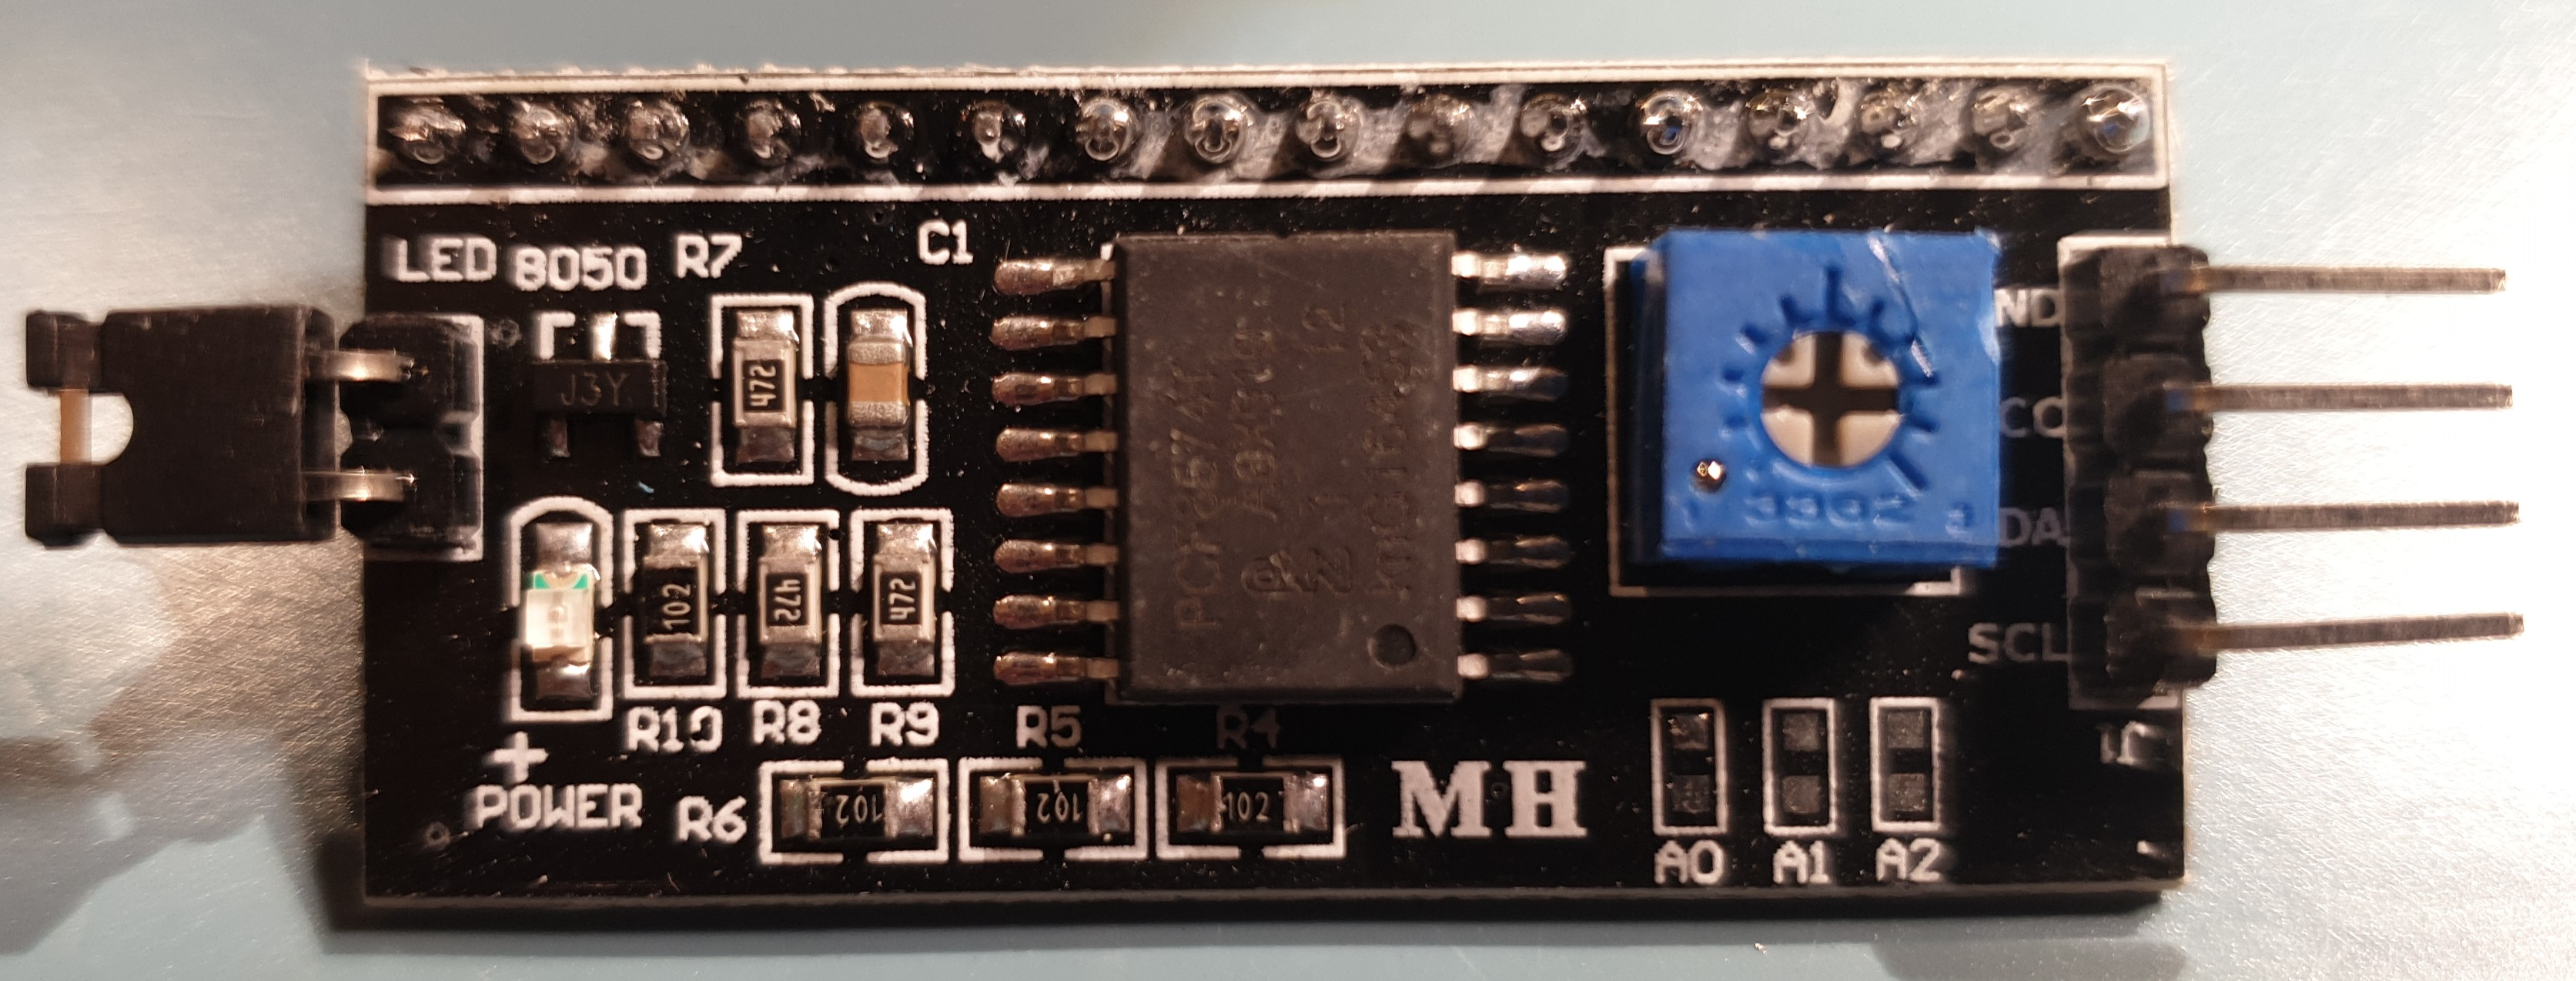
\includegraphics[width=0.45\textwidth]{PCB-LCD-modul-pred}
    }
    \subcaptionbox{Modul po modifikaci}{%
        \includegraphics[width=0.45\textwidth]{PCB-LCD-modul-po}
    }
    \subcaptionbox{%
        Odpájení SMD součástek horkovzdušnou stanicí (poznámka: fotografie byla
        pořízena před aplikací tavidla)
    }{%
        \includegraphics[width=0.80\textwidth]{PCB-LCD-modul-horkovzduska}
    }
    \caption{Modifikace LCD modulu}
    \label{fig:PCB LCD modul modifikace}
\end{figure}


\subsection{Oživování DPS}
Prvotní testy funkčnosti DPS lze provádět před vložením MCU do patice. Záložní
baterii RTC je vhodné vyjmout z držáku, abychom zabránili jejímu vybití častým
spínáním bzučáku~-- ten totiž při zapnutí DPS bez MCU či s MCU bez validního
firmware nepřetržitě píská. Na jednotlivé piny patice můžeme přivádět různé
signály či provádět měření napětí na nich pomocí digitálního multimetru nebo
osciloskopu. Tímto způsobem lze testovat stmívač LED, zvukový výstup, bzučák
indikující ztrátu napájení a tlačítka. Toto ověření funkčnosti není nutné
provádět, je to ale vhodné pro snížení rizika poškození MCU.

Po provedení základních testů vložíme MCU do patice. Nahrání firmware se
provádí pomocí ISP programátoru USBasp připojeného ke konektoru J4. Postup
programování je popsán v souboru \repopath{README.md} repozitáře
\gitrepo{AlarmClock}. Po nahrání firmware by měla DPS být plně funkční, na
hlavní DPS není nutné provádět žádná analogová nastavení. Po připojení LCD je
ale potřeba nastavit jeho kontrast trimrem na desce I/O expandéru PCF8574.

U prvního prototypu bylo provedeno měření s cílem ověřit správnou funkci všech
jeho částí. Digitální signály (sběrnice \IIC{} a UART) byly měřeny logickým
analyzátorem Saleae Logic 16. Stmívač LED byl kontrolován připojením stolního
multimetru do série s LED a zasíláním příkazů pro rozsvěcení s různými
požadovanými hodnotami jasu na rozhraní UART. Kontrolu zvukového výstupu lze
provést připojením osciloskopu paralelně k reproduktoru.

\begin{figure}[htbp]
    \centering
    \includegraphics[width=1.00\textwidth]{PCB-ozivovani-obvod}
    \caption{%
        Kontrola správné funkce DPS budíku s využitím logického analyzátoru
        a~digitálních mutlimetrů
    }
    \label{fig:PCB ozivovani logic}
\end{figure}
\begin{figure}\ContinuedFloat
    \centering
    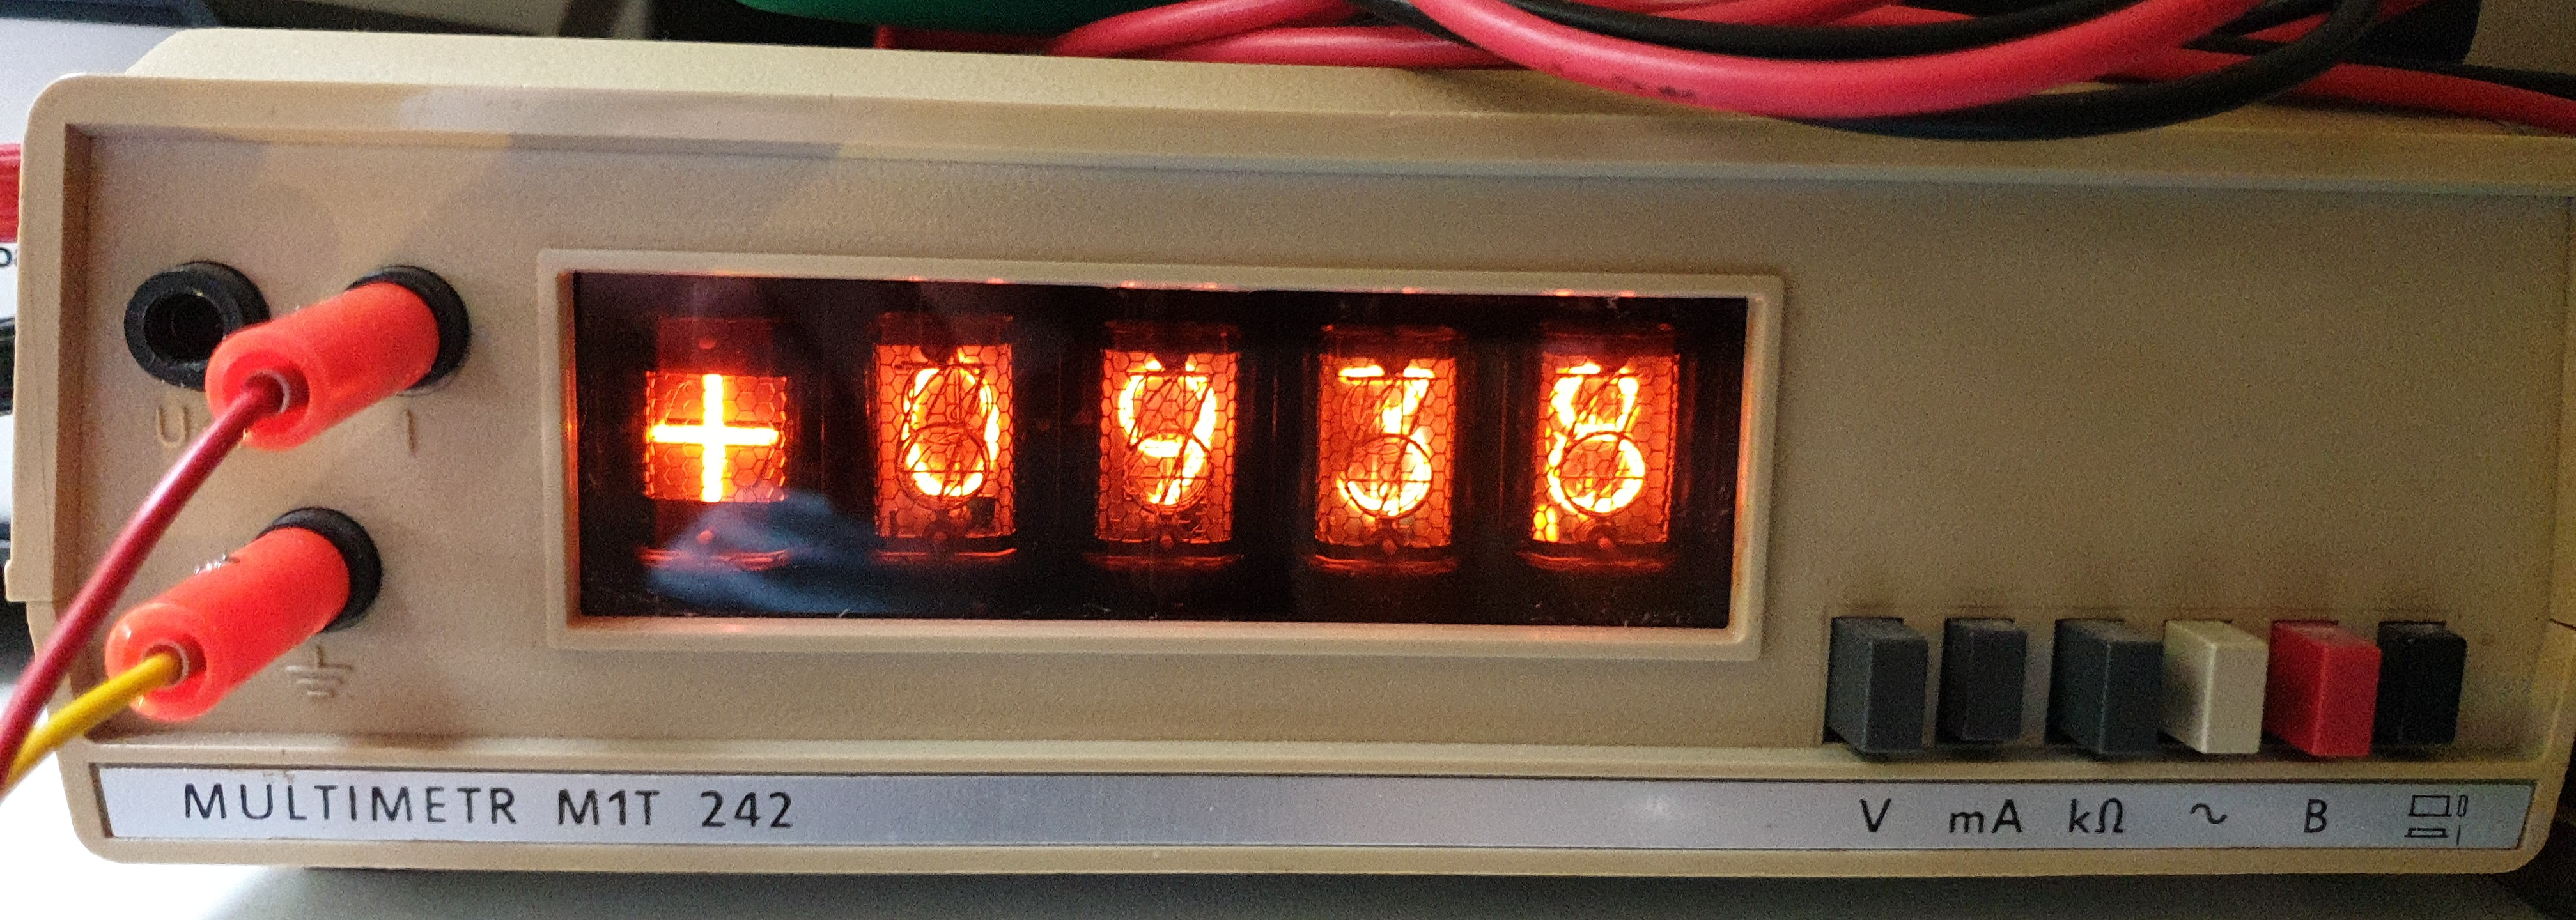
\includegraphics[width=0.90\textwidth]{PCB-ozivovani-metra}
    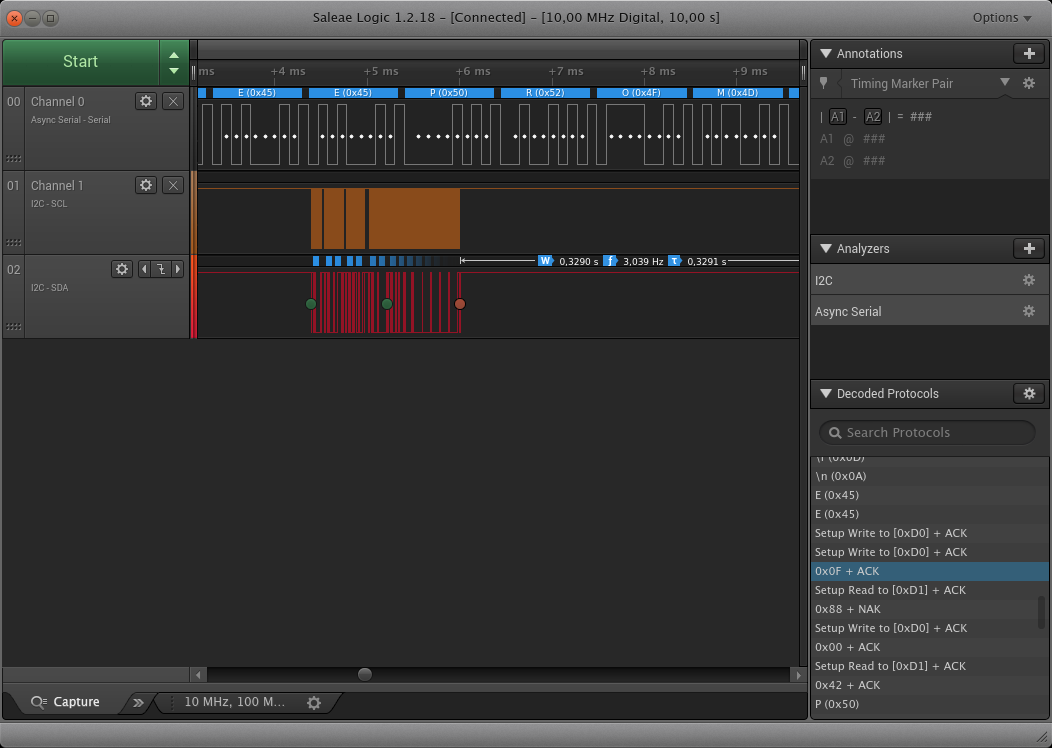
\includegraphics[width=1.00\textwidth]{PCB-ozivovani-logic}
\end{figure}
